\section{The Usual \Luscher Finite-Volume Formalism}\label{sec:formalism/spherical}

The technology and generality of the \Luscher finite-volume formalism has grown substantially \todo{cite cite}.  Here we focus on a simple $s$-wave derivation.

Consider two interacting particles of equal mass $m$.
We assume a pure contact interaction (regulated if needed depending on dimension),
\begin{equation}
V(\vec{r})=C_0(\Lambda)\delta(\vec{r})\ ,
\end{equation}
where $\vec{r}$ represents the relative distance between the two particles and $C_0(\Lambda)$ is the strength of interaction that in principle depends on the regulator and whose units depend on the spatial dimension $d$.  We also assume the system has zero CM motion (i.e. $\vec{P}_{cm}=0$) to make the problem simpler.
The relevant diagram we should calculate in both infinite and finite volume is shown in \Figref{bubbleSum}.

\begin{figure}[ht!]
\center
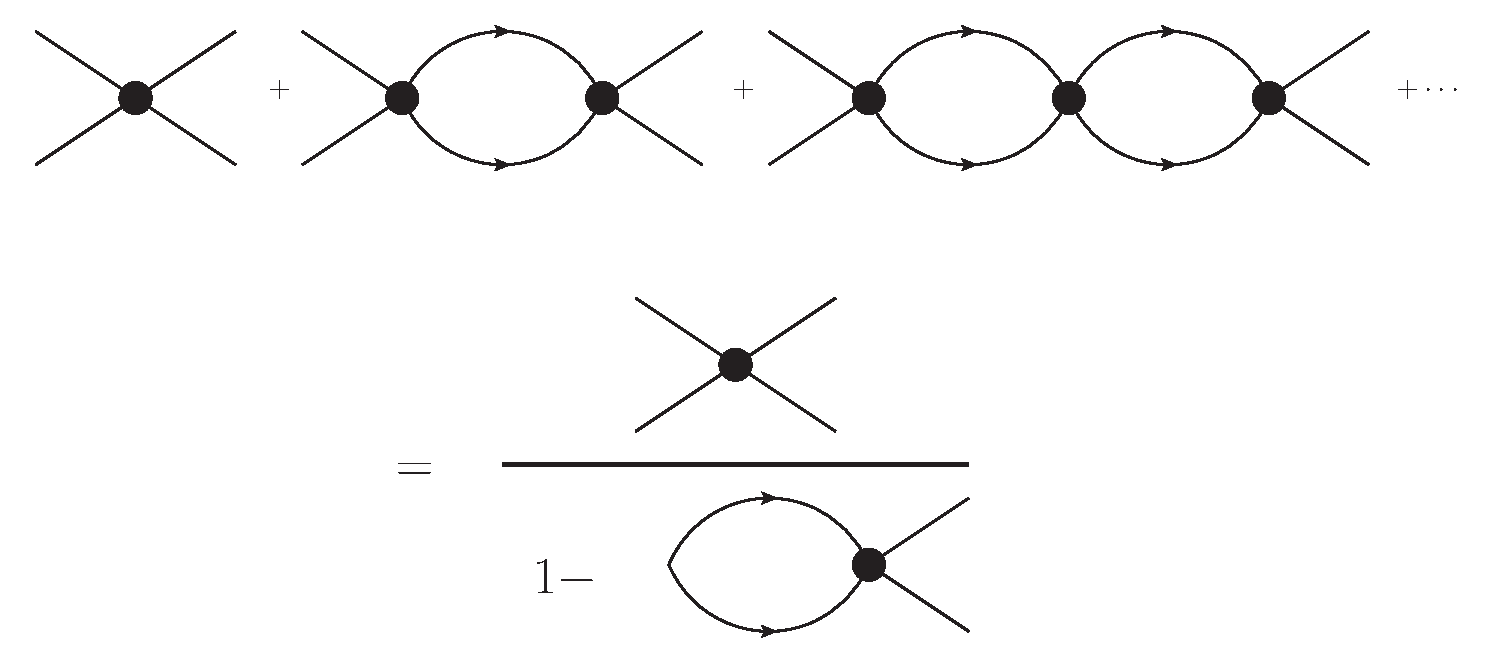
\includegraphics[width=.8\columnwidth]{figure/bubbleSum.eps}
\caption{Bubble sum. Each vertex represents $-iC_0(\Lambda)$ and the bubble represents $I_0$.\label{fig:bubbleSum}}
\end{figure}

This bubble sum is a geometric series and gives\cite{Kaplan:1998we,Beane:2003da}
\begin{equation}\label{eq:scattering amplitude}
\frac{-iC_0(\Lambda)}{1-I_0(p,\Lambda)C_0(\Lambda)}\equiv iT(p)\ ,
\end{equation}
where $T$ is the standard $T$-matrix, $p$ is the relative momentum,  and $I_0(p,\Lambda)$ is a $d$-dependent function described below.  Since we assume a momentum-independent contact interaction, this problem only affects $s$-wave systems, and the $T$-matrix in $D$ spatial dimensions can be related to the s-wave phase shift $\delta_0$ by
\begin{equation}
T=\frac{4}{m}\mathcal{F}_d\frac{1}{\cot \delta_0(p)-i}\ ,
\end{equation}
where
\begin{equation}
\mathcal{F}_D=
\begin{cases}
\pi/p & (D=3)\\
1 & (D=2)\\
p/2 & (D=1)
\end{cases}
\end{equation}
is a dimension-dependent kinematic factor.
Therefore we have
\begin{equation}\label{eq:T matrix matching}
\boxed{
\frac{4}{m}\mathcal{F}_d\frac{1}{\cot \delta_0(p)-i}=\frac{-C_0(\Lambda)}{1-I_0(p,\Lambda)C_0(\Lambda)}
}\ .
\end{equation}
We can recast eq.~\eqref{T matrix matching},
\begin{equation}\label{eq:matching}
\cot \delta_0(p)-i=\frac{4}{m}\mathcal{F}_d\left(\frac{-1}{C_0(\Lambda)}+I_0(p,\Lambda)\right)\ .
\end{equation}
For the special case of a delta function interaction, one has \cite{busch1998}
\begin{equation}\label{eq:phase shifts}
\cot \delta_0(p) =
\begin{cases}
 - \frac{1}{a _ { 0 }p }&\quad (D=3)  \\
\frac { 2 } { \pi } \log \left( p a _ { 0 } \right) & \quad (D=2)\\
 p a _ { 0 } &\quad (D=1)
 \end{cases}\ ,
\end{equation}
where $a_0$ is the scattering length, and the effective range expansion simply adds polynomial terms in $p^2$.
For example, in three dimensions,
\begin{equation}
    \label{eq:ERE}
    p \cot \delta_0(p) = - \frac{1}{a_0} + \frac{1}{2} r_0 p^2 - \frac{1}{4!} s_4 r_0^3 p^4 + \order{p^6},
\end{equation}
where $a_0$ is the scattering length, $r_0$ the effective range, and $s_4$ a higher-order shape parameter.


\begin{figure}[h!]
\center
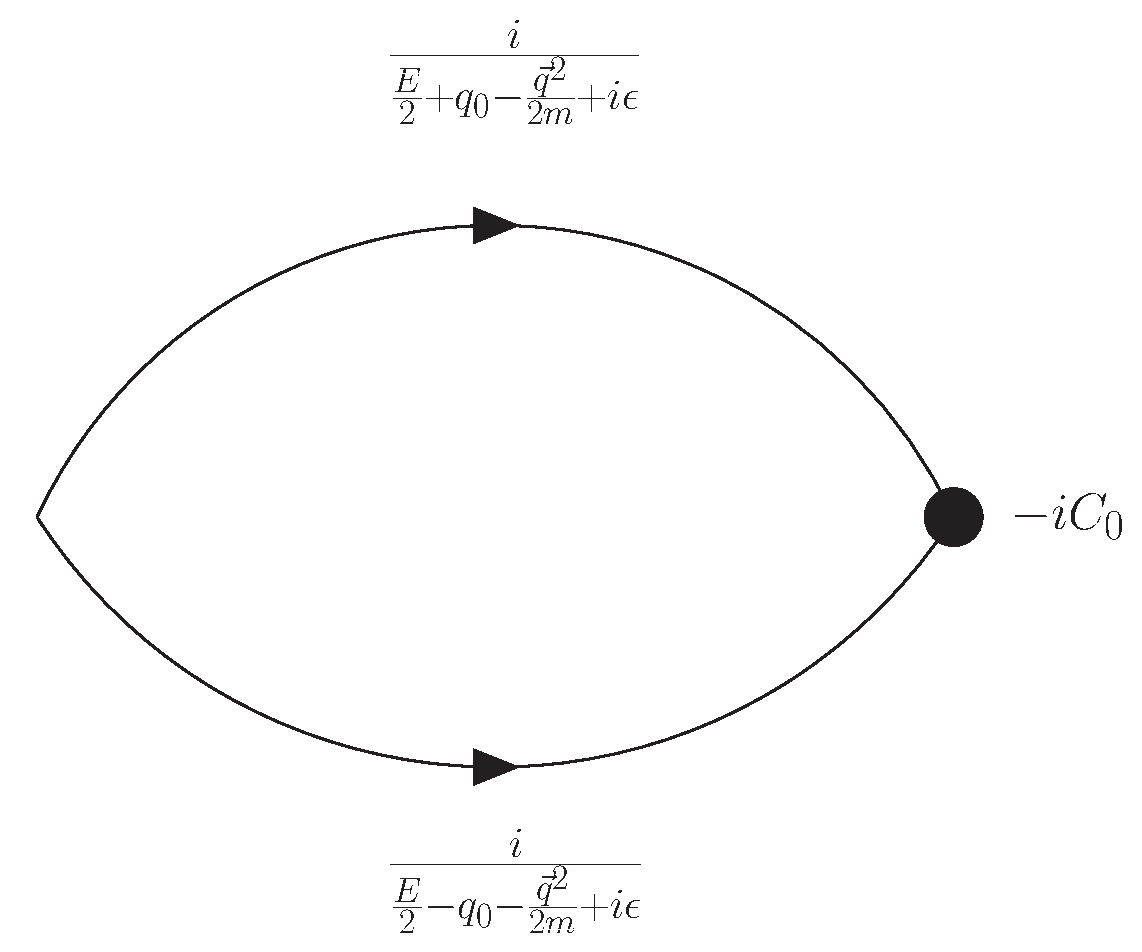
\includegraphics[width=.35\columnwidth]{figure/I0.eps}
\caption{Loop diagram contributing to $I_0$.\label{fig:I0}}
\end{figure}

\subsection{Infinite Volume}

The infinite-volume $I_0(p)$ function is the value of the single bubble, shown in \Figref{I0}.
Standard techniques yield
\begin{align}
    I_0(p)
    &=-i\int^\Lambda \frac { \mathrm {d}q_0 \mathrm { d } ^ { D } \mathbf { q } } { ( 2 \pi ) ^ { D+1 } } \left( \frac { i } { \frac{E}{2} + q _ { 0 } - \frac{\vec{q}^2}{2m} + i \epsilon } \right) \left( \frac { i } { \frac{E}{2} - q _ { 0 } - \frac{\vec{q}^2}{2m} + i \epsilon } \right)
    \nonumber\\
    &=\frac{\Omega_d}{(2\pi)^D}\int^\Lambda  \mathrm { d } q \ q^{D-1}\left[\mathcal{P} \left( \frac { 1 } { E - \frac{\vec{q}^2}{m} } \right)
-i\frac{\pi m}{2q}\delta(q-\sqrt{mE})\right]
    \label{eq:I0}
    \ ,
\end{align}
where $\mathcal{P}$ refers to Principle (Cauchy) Value and the geometric factor
\begin{equation}
\Omega_D=\frac{2\pi^{D/2}}{\Gamma(D/2)}=
\begin{cases}
4\pi&\quad\quad (D=3)\\
2\pi&\quad\quad (D=2)\\
\ 2\ &\quad\quad (D=1)
\end{cases}\ ,
\end{equation}

In three dimensions we must choose a regulator to tame the integral in $I_0$; the coefficient $C_0(\Lambda)$ will depend on this regular such that observables are regulator-independent.  Here we choose a simple, hard cutoff in maximum momentum $\Lambda$, as that matches the lattice calculations we consider.  As with all calculations, we formally take the cutoff to infinity at the end.
Using the on-shell condition $\sqrt{mE}=p$ the $I_0$ becomes
\begin{equation}
    I_0(p) = \frac{1}{2\pi^2}\mathcal{P}\int_0^\Lambda  \mathrm { d } q \ q^2 \left( \frac { 1 } { E - \frac{\vec{q}^2}{m} } \right)
-i\frac{m}{4\pi}p
\end{equation}
which we may plug into \eqref{matching} to find
\begin{equation}
    p\cot \delta_0(p)-ip=\frac{4\pi}{m}\left(\frac{-1}{C_0(\Lambda)}+\frac{1}{2\pi^2}\mathcal{P}\int_0^\Lambda  \mathrm { d } q \ q^2 \left( \frac { 1 } { E - \frac{\vec{q}^2}{m} } \right)\right)-ip\ .
\end{equation}
For general interactions (not just contact interactions) we can determine $C_0(\Lambda)$ by looking at the zero-energy threshold.  Performing the principal-value integral one finds
\begin{align}
    p\cot \delta_0(p)-ip
    &=
    \frac{4\pi}{m}\frac{-1}{C_0(\Lambda)}+\frac{2\Lambda}{\pi} \left(\frac{p}{\Lambda} \tanh ^{-1}\left(\frac{\Lambda }{p}\right)-1 \right)-ip\ ,
    \\
    &p=\frac{4\pi}{m}\left(\frac{-1}{C_0(\Lambda)}-\frac{m\Lambda}{2\pi^2}\right)-ip+\frac{2}{\pi\Lambda}p^2+\frac{2}{3\pi\Lambda^3}p^4+\mathcal{O}(p^6)\ .
\end{align}
where in the second line we have performed a perturbative expansion assuming $p<\Lambda$.  Matching to the effective range expansion \eqref{ERE}
\begin{align}
    -\frac{1}{a_0} &= \frac{4\pi}{m}\left( \frac{-1}{C_0(\Lambda)}-\frac{m\Lambda}{2\pi^2}\right)
    \nonumber
    \\
    r_0 &= +\frac{4}{\pi \Lambda}   &
    (D   &= 3)
    \\
    \nonumber
    s_4 &= -\frac{\pi^2}{4}
\end{align}
and so on, so that we have isolated the scattering length $a_0$, and the cutoff-induced effective range and shape parameters that vanish in the continuum limit.
Solving for $C_0(\Lambda)$ one finds
\begin{equation}
    C_0(\Lambda) = \frac{4\pi/m}{1/a_0 - 2\Lambda/\pi}  \quad\quad (D=3).
\end{equation}

In two dimensions we again use a hard cutoff and match to the effective range expansion, finding
\begin{align}
    p \cot \delta_0(p)
    &=
    \frac{4}{m}\frac{-1}{C_0(\Lambda)} + \frac{2}{\pi} \log \frac{p}{\sqrt{\Lambda^2-p^2}}
    \\
    \frac{2}{\pi} \log(p a_0) +\order{p^2}
    &=
    \frac{4}{m}\frac{-1}{C_0(\Lambda)} + \frac{2}{\pi} \log \frac{p}{\Lambda} + \order{p^2}
\end{align}
so that by matching at zero energy one finds
\begin{equation}
    C_0(\Lambda) = - \frac{2\pi}{m \log a_0 \Lambda} \quad\quad (D=2),
\end{equation}
\todo{Explain a bit about what happens with the log.}

In one dimension evaluating $I_0(p)$ does not require a regulator.
One finds
\begin{align}
    \cot \delta_0(p) - i &= \frac{2p}{m}\frac{-1}{C_0(\Lambda)} - i
    \\
    C_0(\Lambda) &= - \frac{2}{m a_0}.
\end{align}
where $C_0$ is $\Lambda$-independent, as advertised.


\subsection{Finite Volume}

In a finite volume the loop integral that defines $I_0(p)$ in an infinite volume \eqref{I0} becomes a sum over allowed momentum states,
\begin{equation}
    \vec{p} = \frac{2\pi}{L} \vec{n}
\end{equation}
for a triplet of integers $\vec{n}$.  We must evaluate
\begin{align}
I_0(p,L)
    &=-i\int \frac { \mathrm {d}q_0}{2\pi} \frac{1}{L^D}\sum_{\vec{q}}^{\vec{q}^2 < \Lambda^2} \left( \frac { i } { \frac{E}{2} + q _ { 0 } - \frac{\vec{q}^2}{2m} + i \epsilon } \right) \left( \frac { i } { \frac{E}{2} - q _ { 0 } - \frac{\vec{q}^2}{2m} + i \epsilon } \right)
    \\
    &=\frac{1}{L^D}\sum_{\vec{q}}^{\vec{q}^2 < \Lambda^2} \frac { 1 } { E - \frac{\vec{q}^2}{m} } \ .
\end{align}
where the magnitude of $\vec{q}$ is cut off so as to match the spherical integration in \eqref{I0}.



\subsection{The Quantization Condition}
